\section{背景介绍}
\begin{frame}[t]{研究背景与意义}
    % 20世纪80年代以来,随着金融市场的创新、金融自由化改革和国际间资本的流动,金融市场飞速发展,随之而来的是许多难以用经典理论来解释的价格现象,比如房地产和股票价格远远脱离其价值的急速膨胀,经济学家称之为“泡沫”。
    \begin{definition}[金融泡沫]
        金融“泡沫”即在现代信用体系下,金融资产的流通价格偏离标的物公允价值的非理性增长。
    \end{definition}
    \begin{figure}
        \centering
        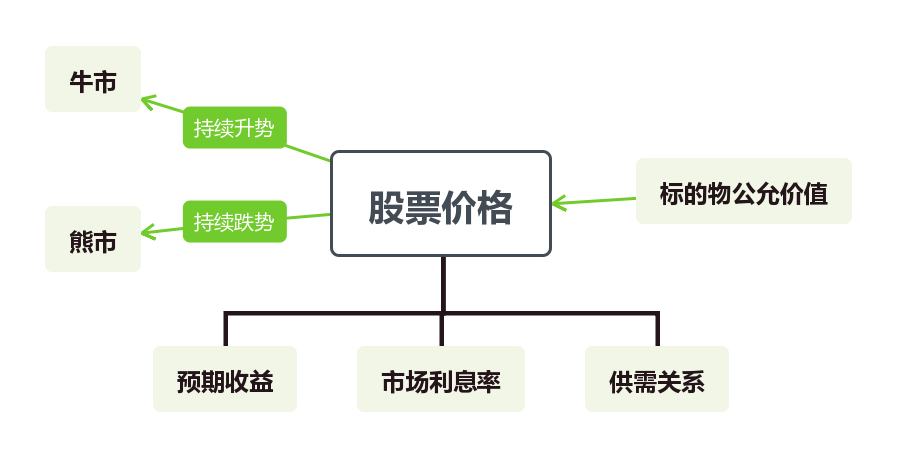
\includegraphics[width=.8\textwidth]{figures/stock}
    \end{figure}
\end{frame}

\begin{frame}[t]{运行规律}
    \begin{enumerate}
        \item 当国民经济向好时,市场参与者对未来经济增长预期良好,金融资产的流通价格趋向于上涨,投资者的收益随之水涨船高;\\[0.5cm]
        \item 在积极的经济预期下这部分收益持续投入资本市场,同时羊群效应促使新的投资者,尤其是中小投资者在市场极度繁荣的吸引下加入市场,创造了新的资本来源,市场价格急速膨胀,开始持续脱离标的物的价值,泡沫产生;\\[0.5cm]
        \item 资产价格飙升到一定程度时,大量投资者纷纷卖出手头的资产以套利,资产供需关系逐渐演变转换,直到价格失去急速上涨的动力,市场的持续繁荣已无法继续维持,价格持续波动导致投资者发现预期与实际相差甚远,市场参与者信心下降,纷纷大面积抛售,情势急转直下直至最后市场崩盘。
    \end{enumerate}
\end{frame}

\begin{frame}[t]{LPPL模型的提出}
    \begin{definition}[LPPL模型对金融泡沫的定义]
        泡沫在这里被定义为资产价格快于指数变动速率的增长现象,反映了积极的高回报预期的反馈螺旋与消极的崩溃预期的反馈螺旋之间的竞争。
    \end{definition}
    \vfill
    为了能够更加准确地预测金融泡沫崩溃点,D.Sornette和A.Johansen基于金融经济学和统计物理学开发了一系列模型和技术,他们发现,市场泡沫行为和地震、物质破裂和其他物理现象存在很多相似之处,都是复杂系统的自组织临界行为。基于这个想法,他们采用复杂科学系统中描述自组织临界现象研究中常用的对数周期性幂律(log-periodic power law, 简称LPPL)来研究金融领域的泡沫现象。
\end{frame}

\begin{frame}[t]{成功预测}
    \begin{enumerate}
        \item 包括2000年--2003 年美国股票市场的反泡沫。
        \item 2004年中期英国的房地产泡沫。
        \item 2008年--2009年中国市场的泡沫。
    \end{enumerate}
    \begin{center}
        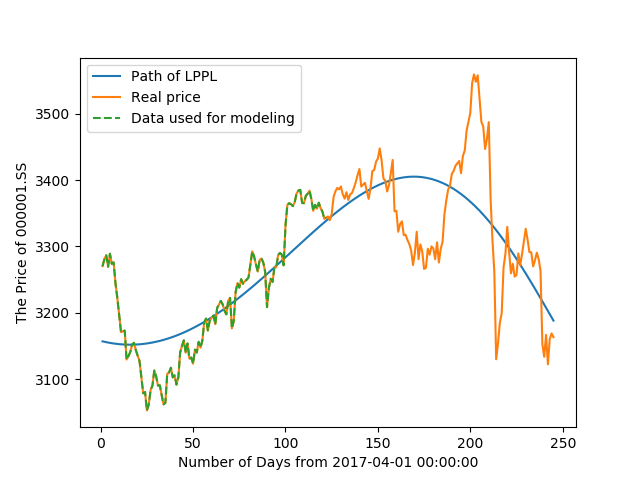
\includegraphics[width=.6\textwidth]{figures/000001SS}
    \end{center}
\end{frame}
